% !TeX root = RJwrapper.tex
\title{MultiStatM: Multivariate Statistical Methods in R}


\author{by György Terdik and Emanuele Taufer}

\maketitle

\abstract{%
The package MultiStatM presents a vectorial approach to multivariate moments and cumulants. Functions provided concern algorithms to build set partitions and commutator matrices, multivariate d-Hermite polynomials; theoretical vector moments and vector cumulants of multivariate distributions and their conversion formulae. Applications discussed concern multivariate measures of skewness and kurtosis; asymptotic covariances for d-variate Hermite polynomials and multivariate moments and cumulants; Gram-Charlier approximations.
}

\hypertarget{introduction-and-background}{%
\section{Introduction and background}\label{introduction-and-background}}

The package \CRANpkg{MultiStatM} (\citet{Taufer22}) provides a set of tools such as set partitions, commutator matrices and vector Hermite polynomials which are needed in developing general computational and conversion formulae for multivariate moments and cumulants of any order. Applications are provided for theoretical moments and cumulants of some important symmetric and skew-symmetric multivariate distributions; measures of multivariate skewness and kurtosis; asymptotic covariance formulae for vector Hermite polynomials; last but not least, estimation functions for all theoretical results discussed are provided. All the methods implemented in \CRANpkg{MultiStatM} are discussed in detail in \citet{terdik2021multivariate}.

A careful study of the cumulants is a necessary and typical part of nonlinear statistics.
Dealing with cumulants for multivariate distributions is made complicated by
the index notations: \citet{mccullagh2018tensor} provides quite an elegant approach using tensor methods; however, tensor methods are not very well known and computationally not so simple. \citet{kollo2008multivariate} and \citet{mori1994multivariate} provide formulae for cumulants in terms of matrices; however, retaining a matrix structure for all higher-order cumulants leads to high-dimensional matrices with special symmetric structures which are quite hard to follow notionally and computationally. Cumulant matrices, with special attention to the third and fourth order, are ubiquitous in the literature. The use of decompositions and approximations allow for dimensionality reduction and find several statistical applications; see \citet{Loperfido15} and \citet{Loperfido17} for analysis and discussion of skewness and kurtosis matrices and their applications.

\CRANpkg{MultiStatM} offers an alternative method, which we believe is simpler to follow: the higher-order cumulants of the same degree for some random \(d\)-vector \(\mathbf{X}\) are collected together and kept as a vector (see \citet{terdik2003higher}). In order to do so, a particular differential operator on a multivariate function, called the \(\operatorname{T}\)-derivative, is introduced. Although the tensor product of Euclidean vectors is not commutative, it has the advantage of permutation equivalence and allows one to obtain general formulae for cumulants and moments of any order. Methods based on a matrix approach do not provide this type of result; see also \citet{ould2015concise}, which goes at most up to the sixth-order moment matrices, whereas there is no such limitation in our derivations and formulae. The vectorial approach has also been advocated by \citet{Holmquist96} and \citet{Chacon2014}; for further discussion, one can see also \citet{kolda2009tensor} and \citet{qi2006rank}.

More formally, with the symbol \(\otimes\) denoting the Cartesian tensor product, consider the operator \(D_{\boldsymbol{\lambda}}^{\otimes}\),
which we refer to as the
\(\operatorname{T}\)-derivative; see \citet{TerdikRaosSankhya06} for details. For any function \({\phi}(\boldsymbol{\lambda})\), the \(\operatorname{T}\)-derivative is defined as
\begin{equation}\label{Tderiv}
D_{\boldsymbol{\lambda}}^{\otimes}{{\phi}}%
(\boldsymbol{\lambda})=\operatorname{vec}\left(\left(  \frac{\partial{\phi
}(\boldsymbol{\lambda})}{\partial\boldsymbol{\lambda}'}\right)'  \right)={\phi}(\boldsymbol{\lambda})\otimes\frac{\partial}{\partial
\boldsymbol{\lambda}}.%
\end{equation}
If \({{\phi}}\) is \(k\)-times differentiable, its \(k\)-th
\(\operatorname{T}\)-derivative is simply
\(D_{\boldsymbol{\lambda}}^{\otimes k}{{\phi} }(\boldsymbol{\lambda})=D_{\boldsymbol{\lambda}}^{\otimes}\left( D_{\boldsymbol{\lambda}}^{\otimes k-1}{{\phi} }(\boldsymbol{\lambda})\right)\). When \({{\phi}}\) is the characteristic function of some random \(d\)-vector, \(k\)-times application of the \(\operatorname{T}\)-derivative will allow to retrieve the so-called multivariate \(\operatorname{T}\)-moments vector of order \(k\), which lists all moments of the same order and has dimension \(d^k\). In the same way, multivariate \(\operatorname{T}\)-cumulants and \(\operatorname{T}\)-Hermite polynomials can be derived. \CRANpkg{MultiStatM} aims at exploiting the advantages of this method for multivariate analysis and dealing with the high-dimensionality implied by this approach.

We could not find any \CRANpkg{R} (\citet{RRR}) package using this approach although there is a partial overlapping between functions in \CRANpkg{MultiStatM} and functions that can be found in other \CRANpkg{R} packages; when this happens, the functions in \CRANpkg{MultiStatM} provide useful generalizations.

The package \CRANpkg{arrangements} (\citet{Lai20}) provides, among other things, all possible partitions of a set (or an integer) in lexicographical order. In \CRANpkg{MultiStatM} all possible partitions in terms of partition matrices together with information about types, sizes and groups of partitions are given. Furthermore \CRANpkg{MultiStatM} provides other partition functions which produce indecomposable partitions, partitions that bring to a closed graph, partitions in only two groups.

The package \CRANpkg{matrixcalc} (\citet{Novom21}) provides the commutation, elimination and duplication matrices for Cartesian tensor products of two vectors, which are particular cases of those provided in the package \CRANpkg{MultiStatM}. Furthermore, in \CRANpkg{MultiStatM} a commutator matrix for any T-product of vectors of any size is given; also, a fast algorithm to produce a symmetrizer of T-products of vectors is implemented (see \citet{Holmquist96}). One of the problems of commutators matrices is their high-dimensionality which can become soon quite cumbersome; on the other hand, commutator matrices are useful if one needs to work with linear combinations of matrices. To deal with the high-dimensionality issue, index versions of the commutators are also provided (more details below).

The package \CRANpkg{calculus} (\citet{guidotti22}) dealing with high dimensional numerical and symbolic calculus provides, up to a given order, the list of all symbolic entries of the multivariate Hermite polynomials with given covariance matrix used here. \CRANpkg{MultiStatM} does not deal with single symbolic expressions rather provides full numerical evaluation of multivariate T-Hermite polynomials suitable for immediate use in further formulas and applications.

\CRANpkg{kStatistics} (\citet{dinardo22a}) gives string expressions for converting single entries of multivariate cumulants or moments which need to be joined and evaluated for numerical computations, for details and examples see \citet{dinardo22b}. This differs to a large degree from the formulae provided in \CRANpkg{MultiStatM} which are always in numerical form and ready for applications; for example, conversion of multivariate moments to multivariate cumulants and viceversa, given any list of (numerical) multivariate moments up to order \(r\), or multivariate cumulants up to order \(r\) are provided.

In \CRANpkg{MultiStatM}, exploiting the conversion formulae and some results on uniform spherical and folded multivariate normal distributions due to \citet{jamma2021San} and \citet{terdik2021multivariate}, the multivariate moments and cumulants of any order of the multivariate skew normal and its generalization (\citet{azzalini1996multivariate} , \citet{arellano2005fundamental}) are provided. The package \CRANpkg{sn} (\citet{Azza22}) provides moments and cumulants of any order for the univariate skew-normal and the skew-t distributions; statistical methods are provided for data fitting and model diagnostics, in the univariate and the multivariate case. In \CRANpkg{MultiStatM} random numbers generator for multivariate skew distributions are provided also.

The package \CRANpkg{moments} (\citet{Komsta22}) deals with functions to calculate, cumulants, Pearson's kurtosis, Geary's kurtosis and skewness; tests related to them from univariate data. However the multivariate approach is not considered. The packages \CRANpkg{mpoly} (\citet{khale13}) and \CRANpkg{orthopolynom} (\citet{Novom22}) deal with Hermite polynomials in the univariate case.

\CRANpkg{MultiStatM} provides some common measures of cumulant-based multivariate skewness and kurtosis (\citet{Mardia70}, \citet{mori1994multivariate}) which are provided in a number of packages, for example \CRANpkg{MaxSkew} (\citet{LoperfidoMax}), \CRANpkg{MultiSkew} (\citet{LoperfidoMus}) and \CRANpkg{Kurt} (\citet{loperfido21}). Indeed the vectorial approach provides a unifying framework for several cumulant-based skewness and kurtosis indexes, as discussed in \citet{jamma2021San} where, beyond the above mentioned ones, indexes proposed by \citet{malkovich1973}, \citet{kollo2008multivariate}, \citet{koziol1987}, \citet{koziol1989} and others are discussed. When going higher than the fourth order, the vectorial approach shows it full power; see \citet{jamma2021SJS} for an application in deriving the asymptotic variances of skewness and kurtosis vectors and indexes which require cumulants up to the \(8\)-th order. Below, exploiting \CRANpkg{MultiStatM} applications to the construction of new measures of multivariate skewness and kurtosis and derivation of Gram-Charlier approximation to densities will be presented.

As far as non R-universe is concerned, the proprietary software Mathematica (\citet{Mathematica}) provides partial overlapping of the multivariate methods discussed in \CRANpkg{MultiStatM}. There, functions to compute, numerically and symbolically, multivariate moments and cumulants of common distributions and general conversion functions from moments to cumulants and viceversa are available. Most of the multivariate distributions discussed in \CRANpkg{MultiStatM} however are not available there. Mathematica also provides several functions for univariate Hermite polynomials which however need to be adapted for the multivariate case based on the \(\operatorname{T}\)-derivative approach.

\hypertarget{package-features}{%
\section{Package features}\label{package-features}}

\CRANpkg{MultiStatM} imports \CRANpkg{arrangements}, \CRANpkg{MASS} (\citet{Mass02}), \CRANpkg{Matrix} (\citet{Matrix24}), \CRANpkg{mvtnorm} (\citet{MVT09}) and \CRANpkg{stats}. We discuss here some examples on the use of the functions; considerations about timing, objects size and algorithms will be collected in Section 4.

\hypertarget{set-partitions}{%
\subsection{Set partitions}\label{set-partitions}}

\CRANpkg{MultiStatM} provides several functions dealing with set partitions. Such functions provide some basic tools used to build the multivariate formulae for moments and cumulants in the following sections.

Generally a set of \(N\) elements can be split into a set of disjoint subsets, i.e.~it can be partitioned. The set of \(N\) elements will correspond to set \(1 : N = \{1, 2, \dots ,N\}\). If \({\cal{K}} = \{b_1, b_2, \dots , b_r \}\) where each \(b_j \subset 1 : N\), then \({\cal{K}}\) is a partition provided
\(\cup b_j = 1 : N\), each \(b_j\) is non-empty and \(b_j \cap b_i = \emptyset\) (the empty set) is disjoint
whenever \(j \neq i\). The subsets \(b_j\), \(j = 1, 2, \dots, r\) are called the blocks of \(\cal{K}\). We
will call \(r\) (the number of the blocks in partition \(\cal{K}\)), the size of \(\cal{K}\), and denote it by \(|{\cal{K}}| = r\), and a partition with size \(r\) will be denoted by \({\cal{K}}_{\{r\}}\). Let us denote the set
of all partitions of the numbers \(1 : N\) by \({\cal{P}}_N\).

Consider next a partition \({\mathcal{K}}_{\{r\}}=\{b_{1},b_{2},\dots,b_{r}\}\in {\mathcal{P}}_{N}\), with size \(r\). Denote the cardinality \(k_{j}\)
of a block in the partition \({\mathcal{K}}_{\{r\}}\), i.e.~\(k_{j}=|b_{j}|\).
The type of a partition \({\mathcal{K}}_{\{r\}}\) is \(l=[l_{1},\dots ,l_{N}]\),
if \({\mathcal{K}}_{\{r\}}\) contains exactly \(l_{j}\) blocks with cardinality \(j\). The type \(l\) is with length \(N\) always. A partition with size \(r\) and
type \(l\) will be denoted by \({\mathcal{K}}_{\{r|l\}}\). It is clear that
\(l_{j}\geq 0\), and \(\sum_{j}jl_{j}=N\), and \(\sum_{j}l_{j}=r\). Naturally, some
\(l_{j}\)'s are zero. A block constitutes a row vector of entries \(0\)'s and \(1\)'s with length \(N\). The places of \(1\)'s correspond to the elements of the block. A partition matrix collects the rows of its blocks, it is an \(r\times N\) matrix with column-sums \(1\).

The basic function is \texttt{PartitionTypeAll} which provides complete information on the partition of a set of \texttt{N} elements, namely:

\begin{itemize}
\item
  \texttt{S\_N\_r}: a vector with the number of partitions of size \texttt{r=1}, \texttt{r=2}, etc. (Stirling numbers of the second kind); \texttt{S\_N\_r{[}r{]}} denotes the number of partition matrices
  of size \texttt{r}.
\item
  \texttt{Part.class}: the list of all possible partitions given as partition matrices. This list is enumerated according to \texttt{S\_N\_r{[}r{]}}, \(r=1,2,\ldots N\), such that the partition matrices with
  size \texttt{R} are listed from \(\sum_{r<R}\)\texttt{S\_N\_r}\(\left[ r\right] +1\) up to \(\sum_{r\leq R}\)\texttt{S\_N\_r}\(\left[ r\right]\). The order of the
  partition matrices within a fixed size is called canonical.
\item
  \texttt{S\_r\_j}: a list of vectors of number of partitions with given types grouped by partitions of size \texttt{r=1}, \texttt{r=2}, etc.; an entry is the number of partitions with that type.
\item
  \texttt{eL\_r}: a list of partition types with respect to partitions of size \texttt{r=1}, \texttt{r=2}, etc. ; since a partition type is a row
  vector with length \texttt{N} this list includes matrices of types (row vectors), the number of rows are the length of vectors of \texttt{S\_r\_j} of a given size \texttt{r}.
\end{itemize}

\textbf{Example 1}. Consider the case where \texttt{N=4} and run the following

\begin{verbatim}
PTA <- PartitionTypeAll(4)
\end{verbatim}

\texttt{S\_N\_r} provides the number of partitions with \texttt{r=1} to \texttt{r=4} blocks:

\begin{verbatim}
PTA$S_N_r
\end{verbatim}

\begin{verbatim}
#> [1] 1 7 6 1
\end{verbatim}

From the results above we see that there are: 1 partition of 1 block (\texttt{r=1}); 7 partitions of two blocks (\texttt{r=2}); 6 partitions of 3 blocks and 1 partition of 4 blocks.
All the partition matrices are listed in \texttt{Part.class}, for example the first partition matrix of size 2 among 7 is

\begin{verbatim}
PTA$Part.class[[2]]
\end{verbatim}

\begin{verbatim}
#>      [,1] [,2] [,3] [,4]
#> [1,]    1    1    1    0
#> [2,]    0    0    0    1
\end{verbatim}

The second partition matrix of size 3 is

\begin{verbatim}
PTA$Part.class[[10]] 
\end{verbatim}

\begin{verbatim}
#>      [,1] [,2] [,3] [,4]
#> [1,]    1    0    1    0
#> [2,]    0    1    0    0
#> [3,]    0    0    0    1
\end{verbatim}

etc.. If one interested in the number of partitions with different types for \texttt{r=2} then consider the list \texttt{S\_r\_j}, i.e.

\begin{verbatim}
PTA$S_r_j[[2]] 
\end{verbatim}

\begin{verbatim}
#> [1] 4 3
\end{verbatim}

That is, for partitions with \texttt{r=2} blocks, there are 2 possible types with 4 and 3 partitions each. These types will show up in the list \texttt{eL\_r}:

\begin{verbatim}
PTA$eL_r
\end{verbatim}

\begin{verbatim}
#> [[1]]
#> [1] 0 0 0 1
#> 
#> [[2]]
#>      [,1] [,2] [,3] [,4]
#> [1,]    1    0    1    0
#> [2,]    0    2    0    0
#> 
#> [[3]]
#> [1] 2 1 0 0
#> 
#> [[4]]
#> [1] 4 0 0 0
\end{verbatim}

From \texttt{PTA\$eL\_r{[}{[}2{]}{]}}
we see that there are two types of partition with \texttt{r=2}: the first is
of type \(\left[ 1,0,1,0\right] ={(l_{1}=1,l_{2}=0,l_{3}=1,l_{4}=0)}\) with 4 partitions and the second is of type \(\left[ 0,2,0,0\right] ={(l_{1}=0,l_{2}=2,l_{3}=0,l_{4}=0)}\) with 3 partitions.

Another general function in this class is \texttt{Partitions} which has a \texttt{Type} argument in order to specify the type of partition to compute: \texttt{2Perm} which provides the permutation of \texttt{N} elements according to a partition matrix \texttt{L}; \texttt{Diagram} which provides the list of partition matrices indecomposable with respect to L, representing diagrams without loops;
\texttt{Indecomp}, which provides the list of all indecomposable partitions with respect to a partition matrix \texttt{L}; \texttt{Pairs}, which provides the list of partitions dividing into pairs the set of \texttt{N} elements.

\hypertarget{commutators-symmetrizer-and-selection-matrices}{%
\subsection{Commutators, symmetrizer and selection matrices}\label{commutators-symmetrizer-and-selection-matrices}}

The \texttt{Commutators} family of functions produce commutators and selection matrices. The use of matrices allows to use linear combinations to represent problems such as the permutation of powers of \(\operatorname{T}\)-products or the selection of certain elements in a vector. On the other hand, the size of these matrices can quickly become quite important. To deal with this issues an option for sparse matrices is always provided; also, a corresponding \texttt{Indx} group of functions which give equivalent results to the corresponding functions in the group \texttt{Matr} is provided.

Two general functions in this family are \texttt{CommutatorMatr} and \texttt{CommutatorIndx}, both with a \texttt{Type} argument selected from: \texttt{Kmn}, \texttt{Kperm}, \texttt{Mixing}, \texttt{Moment}. \texttt{Kmn} produces a commutation matrix, with usual notation \(\mathbf{K}_{m \cdot n}\), of dimension \(mn \times mn\) such that, given a matrix \(\mathbf{A}\) \(m\times n\), \(\mathbf{K}_{m \cdot n} \operatorname{vec}\mathbf{A}=\operatorname{vec}\mathbf{A}'\) (see \citet{terdik2021multivariate}, p.8) while \texttt{Kperm} produce any permutation of Kronecker products of vectors of any length.

\textbf{Example 2}. Consider the product of vectors \(\mathbf{a}_1 \otimes \mathbf{a}_2 \otimes\mathbf{a}_3\) of dimensions \(d_1\) to \(d_3\) respectively.

\texttt{CommutatorMatr(Type="Kperm",c(3,1,2),c(d1,d2,d3))} produces \(\mathbf{a}_3 \otimes \mathbf{a}_1 \otimes\mathbf{a}_2\).

\begin{verbatim}
a1 <- c(1, 2)
a2 <- c(2, 3, 4)
a3 <- c(1, 3)
x <- a1 %x% a2 %x% a3
c(CommutatorMatr(Type = "Kperm", c(3, 1, 2), c(2, 3, 2)) %*% x)
\end{verbatim}

\begin{verbatim}
#>  [1]  2  3  4  4  6  8  6  9 12 12 18 24
\end{verbatim}

\begin{verbatim}
a3 %x% a1 %x% a2
\end{verbatim}

\begin{verbatim}
#>  [1]  2  3  4  4  6  8  6  9 12 12 18 24
\end{verbatim}

The same result can be obtained by using \texttt{CommutatorIndx}

\begin{verbatim}
x[CommutatorIndx(Type = "Kperm", c(3, 1, 2), c(2, 3, 2))]
\end{verbatim}

\begin{verbatim}
#>  [1]  2  3  4  4  6  8  6  9 12 12 18 24
\end{verbatim}

Note that in the example above \texttt{CommutatorMatr} produces the matrix \(\mathbf{K}_{{p}}\) of dimension 12 \(\times\) 12 by which \(\mathbf{y}=\mathbf{K}_{{p}} \mathbf{x}\), while \texttt{CommutatorIndx} produces the permutation \({p}_{\mathbf{y}}\) of 1:12 such that \(\mathbf{y}=\mathbf{x}[{p}_{\mathbf{y}}]\).
Recall that from computational point of view \texttt{CommutatorIndx} is always preferable however, if working with linear combinations of matrices, like in Example 3 and in Section 3.1 and the discussion leading to formulae \eqref{eq:LTA} and \eqref{eq:LTB}, the use of \texttt{CommutatorMatr} is unavoidable. For this reason \CRANpkg{MultiStatM} offers both possibilities. The idea of avoiding the use of commutator, selection (and symmetrizer) matrices can be traced back to \citet{Chacon2014}.

The Elimination and Qplication matrices- related functions respectively eliminate and restore duplicated or q-plicated elements in powers of T-products. For examples of applications of these functions we defer to Section 2.4.

The symmetrizer matrix, a \(d^n \times d^n\) matrix for the symmetrization of a \(\operatorname{T}\)-product of \(n\) vectors with the same dimension \(d\) which overcomes the difficulties arising from the non commutative property of the Kronecker product, and simplifies considerably the computation formulae for multivariate polynomials and their derivatives (see Holmquist (1996) for details). The symmetrizer for a \(\operatorname{T}\)-product of \(q\) vectors of dimension \(d\) is defined as
\begin{equation}
\mathbf{S}_{d \mathbf{1}q}=\frac{1}{q!} \sum_{p \in {\cal{P}}_q} \mathbf{K}_p
\label{eq:DefSym}
\end{equation}
where \({\cal{P}}_q\) is the set of all permutations of the numbers \(1:q\) and \(\mathbf{K}_p\) is the commutator matrix for the permutation \(p \in \cal{P}_q\), (i.e.~the \texttt{CommutatorMatr} with \texttt{Type="Kperm"} of the package). For an application of the symmetrizer via \texttt{SymMatr} with \(d\)-variate Hermite polynomials, see formula \eqref{eq:RecFHP} and Example 3. We defer to Section 4 for a discussion about computational time and memory allocation of these matrices.

\hypertarget{multivariate-t-hermite-polynomials}{%
\subsection{Multivariate T-Hermite polynomials}\label{multivariate-t-hermite-polynomials}}

Consider a Gaussian vector \(\mathbf{X}\) of dimension \(d\) with \(\operatorname{E}\mathbf{X}=0\) and \(\mathbf{\Sigma}=\operatorname{Cov}(\mathbf{X})=\operatorname{E}\mathbf{X X}'\) and define the generator function
\begin{equation}
\begin{split}
\psi(\mathbf{X}; \mathbf{a})&=\exp \left(\mathbf{a}'\mathbf{X} - \frac{1}{2} \mathbf{a}' \mathbf{\Sigma} \mathbf{a}\right) \\
&=\exp \left(\mathbf{a}'\mathbf{X}  - \frac{1}{2} \boldsymbol{\kappa}_2^{\otimes\prime}  \mathbf{a}^{\otimes 2} \right) \\
\end{split}
\end{equation}
where \(\mathbf{a}\) is a \(d\)-vector of constants and \(\boldsymbol{\kappa}_2^{\otimes}=\operatorname{vec}\mathbf{\Sigma}\). The vector Hermite polynomials is defined via the \(\operatorname{T}\)-derivative of the generator function, viz.
\[
\mathbf{H}_n(\mathbf{X}) = D_\mathbf{a}^{\otimes n}\psi(\mathbf{X};\mathbf{a})\big|_{\mathbf{a}=0}.
\]
For example one has
\[
\mathbf{H}_1(\mathbf{X})=\mathbf{X},    \quad \mathbf{H}_2(\mathbf{X})=\mathbf{X}^{\otimes 2} - \boldsymbol{\kappa}_2^{\otimes}.
\]
Note that the multivariate \(\operatorname{T}\)-Hermite polynomial \(\mathbf{H}_n(\mathbf{X})\) is a vector of dimension \(d^n\) which contains the \(n\)-th order polynomials of the vector \(\mathbf{X}^{\otimes n}\). For example the entries of \(\mathbf{H}_2(\mathbf{X})\) are the second order Hermite polynomials \(H_2(X_i,X_j)\), \(i,j=1,2, \dots d\); for \(d=2\)
\[
\mathbf{H}_2(\mathbf{X}) = \left( (X_1^2 - \sigma_{11}), (X_1 X_2 - \sigma_{12}), (X_2 X_1 - \sigma_{21}), (X_2^2 - \sigma_{22})\right)^\prime.
\]
Note that \(\mathbf{H}_n(\mathbf{X})\) is \(n\)-symmetric, i.e.~\(\mathbf{H}_2(\mathbf{X}) = \mathbf{S}_{d \mathbf{1}_n} \mathbf{H}_2(\mathbf{X})\)
where \(\mathbf{S}_{d \mathbf{1}_n}\) is the symmetrizer defined in \eqref{eq:DefSym}. From this one can get useful recursion formulae
\begin{equation}
\mathbf{H}_n(\mathbf{X})=\mathbf{S}_{d \mathbf{1}_n}\left(  \mathbf{H}_{n-1}(\mathbf{X}) \otimes \mathbf{X}- (n-1) \mathbf{H}_{n-2}(\mathbf{X}) \otimes \boldsymbol{\kappa}_2^{\otimes} \right).
\label{eq:RecFHP}
\end{equation}
For further details, consult \citet{terdik2021multivariate}, Section 4.5.

The definition of the \(d\)-variate Hermite polynomial requires the variance-covariance matrix \(\mathbf{\Sigma}\) of the vector \(\mathbf{X}\). \texttt{HermiteN} and \texttt{HermiteN2X} with \texttt{Type=c("Univariate","Multivariate")} compute respectively the univariate and \(d\)-variate Hermite polynomials and their inverses up to a given order \texttt{N} evaluated at \texttt{x} for a given covariance matrix \texttt{Sig2}. By default \texttt{Sig2}=\(I_\mathbf{d}\).

\textbf{Example 3}. Consider a vector \(x\) of dimension \(d=2\) and compute the Hermite polynomials up to order \texttt{N}=\(3\) with identity variance matrix \(\mathbf{I}_2\); \texttt{HermiteN(x,3,Type="Multivariate")} will contain the list of \(d\)-variate Hermite polynomials up to order \(3\) at value \(x\).

\begin{verbatim}
x <- c(1, 2)
HN <- HermiteN(x, 3, Type = "Multivariate")
\end{verbatim}

Retrieve the third Hermite polynomial

\begin{verbatim}
HN[[3]]
\end{verbatim}

\begin{verbatim}
#> [1] -2  0  0  3  0  3  3  2
\end{verbatim}

Use now the symmetrizer in matrix form to verify formula \eqref{eq:RecFHP} with \(n=2\). Note that in this case \(\boldsymbol{\kappa}_2^{\otimes}=\operatorname{vec}\mathbf{I}_2\).

\begin{verbatim}
k2 <- c(1, 0, 0, 1)
c(SymMatr(2, 3) %*% (kronecker(HN[[2]], x) - (3 - 1) * kronecker(HN[[1]], k2)))
\end{verbatim}

\begin{verbatim}
#> [1] -2  0  0  3  0  3  3  2
\end{verbatim}

\hypertarget{multivariate-t-moments-and-t-cumulants}{%
\subsection{Multivariate T-moments and T-cumulants}\label{multivariate-t-moments-and-t-cumulants}}

Multivariate moments and cumulants of all orders of a random vector \(\mathbf{X}\) in \(d\)-dimensions, with mean vector \(\boldsymbol{\mu}\) and covariance matrix \(\mathbf{\Sigma}\) can be obtained by applying the \(\operatorname{T}\)-derivative respectively to the characteristic function and the log of the CF. More formally, let \(\boldsymbol{\lambda}\) a \(d\)-vector of real constants; \(\phi_{\mathbf{X}}(\boldsymbol{\lambda})\) and \(\psi_{\mathbf{X}}(\boldsymbol{\lambda})=\log\phi_{\mathbf{X}}(\boldsymbol{\lambda})\) denote, respectively, the characteristic function and the cumulant function of \(\mathbf{X}\). Then the \(k\)-th order moments and cumulants of the vector \(\mathbf{X}\) are obtained as
\[
\boldsymbol{\mu}^\otimes_{\mathbf{X},k} =   (-\mathbf{i})^k D_{\boldsymbol{\lambda}}^{\otimes k}{{\phi}%
}_{\mathbf{X}}(\boldsymbol{\lambda}) \big|_{\boldsymbol{\lambda}=0}.
\]
\[
\boldsymbol{\kappa}^\otimes_{\mathbf{X},k} =   \underline{\operatorname{Cum}}_k(\mathbf{X})= (-\mathbf{i})^k D_{\boldsymbol{\lambda}}^{\otimes k}{{\psi}%
}_{\mathbf{X}}(\boldsymbol{\lambda}) \big|_{\boldsymbol{\lambda}=0}.
\]
Note that \(\boldsymbol{\mu}_{\mathbf{X},k} = \operatorname{E}\mathbf{X}^{\otimes k}\) is a vector of dimension \(d^k\) that contains all possible moments of order \(k\) formed by \(X_1, \dots, X_d\). This approach has the advantage of being straightforwardly extendable to any \(k\)-th order moment. An analogous discussion can be done for cumulants. Note that one has \(\boldsymbol{\kappa}_{\mathbf{X},2} =\operatorname{vec} \mathbf{\Sigma}\). \CRANpkg{MultiStatM} contains functions which obtains moments from cumulants and vice-versa as well as functions which provide theoretical moments and cumulants for some important multivariate distributions.

The \texttt{Cum2Mom} and \texttt{Mom2Cum} either for the univariate or multivariate cases provide conversion formulae for cumulants from moments and viceversa given any list of moments (or cumulants).

\textbf{Example 4}. Consider the case of the 2-variate standard normal distribution with unit mean vector and covariance matrix with unit elements on the main diagonal and off-diagonal elements equal to 0.5; in this case the first four moments are given in the vector \texttt{mu} below

\begin{verbatim}
mu <- list(
  c(1, 1), c(2, 1.5, 1.5, 2), c(4, 3, 3, 3, 3, 3, 3, 4),
  +c(10, 7, 7, 6.5, 7, 6.5, 6.5, 7, 7, 6.5, 6.5, 7, 6.5, 7, 7, 10)
)
cum <- Mom2Cum(mu, Type = "Multivariate")
cum
\end{verbatim}

\begin{verbatim}
#> [[1]]
#> [1] 1 1
#> 
#> [[2]]
#> [1] 1.0 0.5 0.5 1.0
#> 
#> [[3]]
#> [1] 0 0 0 0 0 0 0 0
#> 
#> [[4]]
#>  [1] 0 0 0 0 0 0 0 0 0 0 0 0 0 0 0 0
\end{verbatim}

Getting back to moments

\begin{verbatim}
Cum2Mom(cum, Type = "Multivariate")
\end{verbatim}

\begin{verbatim}
#> [[1]]
#> [1] 1 1
#> 
#> [[2]]
#> [1] 2.0 1.5 1.5 2.0
#> 
#> [[3]]
#> [1] 4 3 3 3 3 3 3 4
#> 
#> [[4]]
#>  [1] 10.0  7.0  7.0  6.5  7.0  6.5  6.5  7.0  7.0  6.5  6.5  7.0  6.5  7.0  7.0
#> [16] 10.0
\end{verbatim}

If one wishes to select only the distinct moments from the vector of third moments, then

\begin{verbatim}
r.mu <- mu[[3]][EliminIndx(2, 3)]
r.mu
\end{verbatim}

\begin{verbatim}
#> [1] 4 3 3 4
\end{verbatim}

Note that \texttt{EliminIndx} (and \texttt{EliminMatr}) does not correspond to the function \texttt{unique}, rather it individuates the distinct elements from the symmetry of the Kronecker product. Here the values 4 and 3 could appear to be duplicates however in general they could be different. This allows to recover the whole vector when needed by using \texttt{QplicIndx} (or \texttt{QplicMatr})

\begin{verbatim}
mu3 <- r.mu[QplicIndx(2, 3)]
mu3
\end{verbatim}

\begin{verbatim}
#> [1] 4 3 3 3 3 3 3 4
\end{verbatim}

The \texttt{MomCum} functions provide theoretical moments and cumulants for some common multivariate distributions: Skew-normal, Canonical Fundamental Skew-normal (CFUSN), Uniform distribution on the sphere, central folded Normal distribution (univariate and multivariate); for detail on the multivariate formulae used see \citet{jamma2021San}. Some more details on the multivariate distributions considered are reported in the list below.

\begin{itemize}
\item
  A \(d\)-vector \(\mathbf{U}\) having uniform distribution on the sphere \(\mathbb{S}_{d-1}\). Moments and cumulants of all orders are provided for \(\mathbf{U}\) by the function \texttt{MomCumUniS}; the function \texttt{EVSKUniS} can compute moments and cumulants (up to the 4th order), skewness, and kurtosis of \(\mathbf{U}\) (\texttt{Type="Standard"}) and its modulus (\texttt{Type="Modulus"}).
  Recall that any \(d\)-vector, say \(\mathbf{W}\), has a spherically symmetric distribution
  if that distribution is invariant under the group of rotations in
  \(\mathbb{R}^{d}\). This is equivalent to saying that \(\mathbf{W}\) has the
  stochastic representation \(\mathbf{W}=R\mathbf{U}\)
  where \(R\) is a non negative random variable. Moments and cumulants of \(\mathbf{W}\) can be obtained by its stochastic representation as discussed in \citet{jamma2021San}, Theorem 1 and Lemma 1. Furthermore a \(d\)-vector \(\mathbf{X}\) has an elliptically symmetric distribution if it has the representation
  \[
  \mathbf{X}=\boldsymbol{\mu}+\boldsymbol{\Sigma}^{1/2}\mathbf{W},%
  \]
  where \(\boldsymbol{\mu}\in\mathbb{R}^{d}\), \(\boldsymbol{\Sigma}\) is a
  variance-covariance matrix and \(\mathbf{W}\) is spherically distributed.
  Hence the cumulants of \(\mathbf{X}\) are just constant times the cumulants
  of \(\mathbf{W}\) except for the mean i.e.
  \[
  \underline{\operatorname*{Cum}}_{m}\left(  \mathbf{X}\right)  =\left(
  \boldsymbol{\Sigma}^{1/2}\right)  ^{\otimes m}\underline{\operatorname*{Cum}%
  }_{m}\left(  \mathbf{W}\right)  .
  \]
\item
  If \(\mathbf{Z}\) denotes a \(d\)-vector with \(d\)-variate standard normal distribution, the function \texttt{MomCumZabs} provides the moments and cumulants of \(|\mathbf{Z}|\) respectively in the univariate (\texttt{Type="univariate"}) and multivariate case (\texttt{Type="Multivariate"}).
\item
  The multivariate skew-normal distribution introduced by \citet{azzalini1996multivariate}, whose marginal densities
  are scalar skew-normals. A \(d\)-dimensional random vector \(\mathbf{X}\) is
  said to have a multivariate skew-normal distribution, \(\text{SN}_{d}\left(\boldsymbol{\mu},\boldsymbol{\Omega},\boldsymbol{\alpha}\right)\) with shape
  parameter \(\boldsymbol{\alpha}\) if it has the density function
  \[
  2\varphi\left(  \mathbf{X};\boldsymbol{\mu},\boldsymbol{\Omega}\right)
  \Phi\left(  \boldsymbol{\alpha}' \left(  \mathbf{X}-\boldsymbol{\mu
  }\right)  \right)  , \quad\mathbf{X} \in\mathbb{R}^{d},
  \]
  where \(\varphi\left(\mathbf{X};\boldsymbol{\mu},\boldsymbol{\Omega}\right)\) is the \(d\)-dimensional normal density with mean \(\boldsymbol{\mu}\)
  and correlation matrix \(\boldsymbol{\Omega}\); here \(\varphi\) and \(\Phi\) denote
  the univariate standard normal density and the cdf. For a general formula for cumulants, see \citet{jamma2021San}, Lemma 4. For this distribution are available the functions \texttt{MomCumSkewNorm}, which computes the theoretical values of moments and cumulants up to the r-th order and \texttt{EVSKSkewNorm} which gives mean vector, covariance, skewness and kurtosis vectors and other features.
\item
  \citet{arellano2005fundamental} introduced the
  CFUSN distribution (cf.~their Proposition 2.3), to include all
  existing definitions of skew-normal distributions. The marginal stochastic
  representation of \(\mathbf{X}\) with distribution \(\text{CFUSN}_{d,m}\left(\boldsymbol{\Delta}\right)\) is given by
  \[
    \mathbf{X}=\boldsymbol{\Delta}\left\vert \mathbf{Z}_{1}\right\vert
    +\left(  \mathbf{I}_{d}-\boldsymbol{\Delta\Delta}'\right)
    ^{1/2}\mathbf{Z}_{2}, 
  \]
  where \(\boldsymbol{\Delta}\), is the \(d\times m\) skewness matrix such that
  \(\left\Vert \boldsymbol{\Delta}\mathbf{a}\right\Vert <1\), for all
  \(\left\Vert \mathbf{a}\right\Vert =1\), and \(\mathbf{Z}_{1}\in\mathcal{N}\left( 0,\mathbf{I}_{m}\right)\) and \(\mathbf{Z}_{2}\in\mathcal{N}\left( 0,\mathbf{I}_{d}\right)\) are independent (Proposition 2.2. Arellano-Valle and Genton (2005)). A simple construction of
  \(\boldsymbol{\Delta}\) is \(\boldsymbol{\Delta}=\boldsymbol{\Lambda}\left(\mathbf{I}_{m}\mathbf{+}\boldsymbol{\Lambda}' \boldsymbol{\Lambda}\right)^{-1/2}\) with some real matrix \(\boldsymbol{\Lambda}\) with dimensions \(d\times m\). The \(\text{CFUSN}_{d,m}\left(\boldsymbol{\mu},\boldsymbol{\Sigma},\boldsymbol{\Delta}\right)\) can be defined via the linear transformation
  \(\boldsymbol{\mu}+\boldsymbol{\Sigma}^{1/2}\mathbf{X}\). For a general formula for cumulants, see \citet{jamma2021San}, Lemma 5. For this distributions \texttt{MomCumCFUSN} provides moments and cumulants up to the \(r\)-th order.
\end{itemize}

\textbf{Example 5}. For a skew-normal distribution with \(\alpha=(10,5,0)\) and correlation function \(\Omega= \text{diag} (1,1,1)\) the third moments and cumulants are

\begin{verbatim}
alpha <- c(10, 5, 0)
omega <- diag(3)
MSN <- MomCumSkewNorm(r = 3, omega, alpha, nMu = TRUE)
round(MSN$Mu[[3]], 3)
\end{verbatim}

\begin{verbatim}
#>  [1] 1.568 0.073 0.000 0.073 0.570 0.000 0.000 0.000 0.711 0.073 0.570 0.000
#> [13] 0.570 0.996 0.000 0.000 0.000 0.355 0.000 0.000 0.711 0.000 0.000 0.355
#> [25] 0.711 0.355 0.000
\end{verbatim}

\begin{verbatim}
round(MSN$CumX[[3]], 3)
\end{verbatim}

\begin{verbatim}
#>  [1] 0.154 0.077 0.000 0.077 0.039 0.000 0.000 0.000 0.000 0.077 0.039 0.000
#> [13] 0.039 0.019 0.000 0.000 0.000 0.000 0.000 0.000 0.000 0.000 0.000 0.000
#> [25] 0.000 0.000 0.000
\end{verbatim}

As another example, for the uniform distribution on the sphere, the kurtosis vector is:

\begin{verbatim}
EVSKUniS(3, Type = "Standard")$Kurt.U
\end{verbatim}

\begin{verbatim}
#>  [1] -1.2  0.0  0.0  0.0 -0.4  0.0  0.0  0.0 -0.4  0.0 -0.4  0.0 -0.4  0.0  0.0
#> [16]  0.0  0.0  0.0  0.0  0.0 -0.4  0.0  0.0  0.0 -0.4  0.0  0.0  0.0 -0.4  0.0
#> [31] -0.4  0.0  0.0  0.0  0.0  0.0 -0.4  0.0  0.0  0.0 -1.2  0.0  0.0  0.0 -0.4
#> [46]  0.0  0.0  0.0  0.0  0.0 -0.4  0.0 -0.4  0.0  0.0  0.0 -0.4  0.0  0.0  0.0
#> [61] -0.4  0.0  0.0  0.0  0.0  0.0  0.0  0.0 -0.4  0.0 -0.4  0.0 -0.4  0.0  0.0
#> [76]  0.0 -0.4  0.0  0.0  0.0 -1.2
\end{verbatim}

\hypertarget{analyzing-multivariate-skewness-and-kurtosis}{%
\subsection{Analyzing multivariate skewness and kurtosis}\label{analyzing-multivariate-skewness-and-kurtosis}}

A complete picture of multivariate skewness is provided by the third-order \(\operatorname{T}\)-cumulant (skewness vector) of a standardized \(\mathbf{X}\); set \(\mathbf{Y}=\boldsymbol{\Sigma}^{-1/2}(\mathbf{X}-\boldsymbol{\mu})\), then the skewness vector is
\begin{equation}\label{SkewV}
\boldsymbol{\kappa}_{\mathbf{Y},3}^\otimes= \underline{\operatorname{Cum}}_3 \left( \mathbf{Y}\right)=\left(\mathbf{\Sigma}^{-1/2}\right)^{\otimes 3} \boldsymbol{\kappa}_{\mathbf{X},3}^\otimes.
\end{equation}

A definition of skewness which is invariant under shifting and orthogonal transformations or, in other words affine invariant, is provided by the total skewness of \(\mathbf{X}\), i.e.~the square norm of the skewness vector:
\begin{equation}
\gamma_{1,d}=\|\boldsymbol{\kappa}_{\mathbf{Y},3}^\otimes\|^2 = \beta_{1,d}
\end{equation}
where \(\beta_{1,d}\) is Mardia's multivariate skewness index \citep{Mardia70} which coincides with the total skewness \(\gamma_{1,d}\) since the third-order central moments and third-order cumulants are equal. \citet{mori1994multivariate} (MRSz's) skewness vector can also be recovered from the skewness vector as
\begin{equation}
\mathbf{b}(\mathbf{Y})= \left( \operatorname{vec}' \mathbf{I}_d \otimes  \mathbf{I}_d \right)\boldsymbol{\kappa}_{\mathbf{Y},3}^\otimes.
\label{eq:MoriSkew}
\end{equation}
Note that \(\operatorname{vec}' \mathbf{I}_d \otimes \mathbf{I}_d\) is a matrix of dimensions \(d \times d^3\), which contains \(d\) unit values per-row,
whereas all the others are 0; as a consequence, \(\mathbf{b}(\mathbf{Y})\) does not take into account the contribution of cumulants of the type \(\operatorname{Cum}_3 (X_j,X_k,X_l)\), where all the
three indices \(j\), \(k\), \(l\) are different from each other. The corresponding scalar measure of multivariate skewness is \(b(\mathbf{Y}) = \| \mathbf{b}(\mathbf{Y}) \|^2\).

The fourth-order T-cumulant of the standardized \(\mathbf{X}\), i.e.~\(\boldsymbol{\kappa}_{\mathbf{Y},4}^\otimes =\mathbf{H}_4(\mathbf{Y})\), will be called kurtosis vector of \(\mathbf{X}\); its square norm will be called the total kurtosis of \(\mathbf{X}\),
\begin{equation}
\gamma_{2,d}=\| \boldsymbol{\kappa}_{\mathbf{Y},4}^\otimes \|^2.
\end{equation}
Mardia's kurtosis index \(\beta_{2,d}= \operatorname{E}\left( \mathbf{Y}'\mathbf{Y} \right)^2\) ( \citet{Mardia70}) is related to the kurtosis vector by the formula
\[
\beta_{2,d}= \left( \operatorname{vec}' \mathbf{I}_{d^2} \right)\boldsymbol{\kappa}_{\mathbf{Y},4}^\otimes +d(d+2).
\]
A consequence of this is that Mardia's measure does not depend on all the entries of \(\boldsymbol{\kappa}_{\mathbf{Y},4}^\otimes\)
which has \(d(d +1)(d +2)(d +3)/24\) distinct elements, while \(\beta_{2,d}\) includes only \(d^2\) elements among them. We note that if \(\mathbf{X}\) is Gaussian, then \(\boldsymbol{\kappa}_{\mathbf{Y},4}^\otimes=\mathbf{0}\). Note that \citet{koziol1989}, for \(\mathbf{Y}\) and an independent copy \(\tilde{\mathbf{Y}}\), considered \(\operatorname{E}(\mathbf{Y}'\tilde{\mathbf{Y}})^4\) as an index of kurtosis which is the next higher degree analogue of Mardia's skewness index \(\beta_{1,d}\). Note that (see \citet{jamma2021San})
\[
\operatorname{E}(\mathbf{Y}'\tilde{\mathbf{Y}})^4 = \gamma_{2,d}+6 \beta_{2,d}-d^2.
\]

\citet{mori1994multivariate} define what we will call the MRS kurtosis matrix
\[
\mathbf{B}(Y) =\operatorname{E}\left( \mathbf{Y}\mathbf{Y}' \mathbf{Y}\mathbf{Y}' \right) -(d+2)\mathbf{I}_d,
\]
which can be expressed in terms of the kurtosis vector as (note also that \(\operatorname{tr} \mathbf{B}(Y) = \beta_{2,d}\)),
\[
\operatorname{vec}\mathbf{B}(Y) = \left( \mathbf{I}_{d^2}\otimes \operatorname{vec}' \mathbf{I}_d   \right)\boldsymbol{\kappa}_{\mathbf{Y},4}^\otimes.
\]
\(\mathbf{B}(Y)\) got a prominent role in multivariate statistics due to invariant coordinate selection (\citet{tyler2009}), model-based clustering (\citet{pena2010}), and multivariate outlier detection (\citet{ARCHIMBAUD18}). For further connections between \(\boldsymbol{\kappa}_{\mathbf{Y},3}^\otimes\), \(\boldsymbol{\kappa}_{\mathbf{Y},4}^\otimes\) and other measures of skewness and kurtosis, see \citet{terdik2021multivariate}, Section 6 and \citet{jamma2021San}. For \citet{malkovich1973}, where directional measures of multivariate skewness and kurtosis measures are proposed, one can refer to \CRANpkg{MaxSkew}, \CRANpkg{Kurt} and \citet{Loperfido15} for discussions and applications; see also \citet{arevalillo20} and \citet{arevalillo21}.

For examples on computing skewness and kurtosis measures with \CRANpkg{MultiStatM} and relate tests see the following sections.

\hypertarget{estimation}{%
\subsection{Estimation}\label{estimation}}

Estimating functions starting from a vector of multivariate data are available: multivariate Hermite polynomials, moments, cumulants, skewness and kurtosis vectors, Mardia's skewness and kurtosis indexes, MRSz's skewness vector and kurtosis matrices. The \texttt{Estimation} family of functions include \texttt{SampleEVSK}, \texttt{SampleGC}, \texttt{SampleHermiteN}, \texttt{SampleKurt}, \texttt{SampleSkew}, \texttt{SampleMomCum}, see the examples in this and the next section for their application.

The basic estimation method relies on sample averages: given a random sample of \(d\)-vectors \(\mathbf{X}_1, \dots, \mathbf{X}_n\), for any function \(g\) let
\begin{equation}
\widehat{g(\mathbf{X})}= \frac{1}{n}\sum_{i=1}^n g(\mathbf{X}_i).
\label{eq:MomEst}
\end{equation}
To estimate moments of any order \(k=1, \dots, r\) the function \texttt{SampleMomCum} sets \(g(\mathbf{X}_i)=\mathbf{X}_i^{\otimes k}\) in \eqref{eq:MomEst}, while cumulants are obtained from moments via the function \texttt{Mom2Cum}. Options for centering, i.e.~\((\mathbf{X_i}-\bar{\mathbf{X}})\) or scaling (default), i.e.~\(\mathbf{S}^{-1/2}(\mathbf{X_i}-\bar{\mathbf{X}})\), where \(\bar{\mathbf{X}}\) and \(\mathbf{S}\) are the usual sample estimates of mean and variance, are provided. For any sample \(\mathbf{X}_1, \dots, \mathbf{X}_n\) the mean zero and identity covariance matrix data \(\mathbf{Z}_i= \mathbf{S}^{-1/2}(\mathbf{X_i}-\bar{\mathbf{X}})\) can always be obtained using \texttt{MultiStatM::MVStandardize}.

\(d\)-variate Hermite polynomials of any order \(k=1, \dots, N\) are evaluated at standardized data points setting \(g(\mathbf{X}_i)=\mathbf{H}_k(\mathbf{X}_i)\) in \eqref{eq:MomEst}. The estimators in terms of standard Hermite polynomials proved to be useful for finding the asymptotic distribution of skewness and kurtosis estimates, see \citet{jamma2021SJS}. For estimation of skewness and kurtosis vectors, see \citet{terdik2021multivariate} (6.20), p.~331 and (6.28), p.~340. Formulae for evaluating the variance of estimators are also available. For example \texttt{SampleVarianceSkewKurt} provides estimates of the covariance matrix of the data-estimated skewness and kurtosis vectors; see (\citet{terdik2021multivariate}, (6.13) and (6.22)).

\CRANpkg{MultiStatM} does not make use of multivariate k-statistics in estimation. For these one can use \CRANpkg{kStatistics}; for tutorials see \citet{dinardo22b} and \citet{smith2020tutorial}.

\textbf{Example 6}. Consider a multivariate data vector of dimension \(d=3\) and \(n=1000\) from the multivariate skew-normal distribution of Example 5. The estimated first four cumulants are listed in the object \texttt{EsMSN} obtained by \texttt{SampleEVSK}; the corresponding theoretical values are in the object \texttt{ThMSN} obtained by \texttt{MomCumSkewNorm}.

\begin{verbatim}
data <- rSkewNorm(1000, omega, alpha)
EsMSN <- SampleEVSK(data)
ThMSN <- EVSKSkewNorm(omega, alpha)
\end{verbatim}

Compare the distinct elements of the estimated skewness vector and the theoretical ones using \texttt{EliminIndx}.

\begin{verbatim}
EsMSN$estSkew[EliminIndx(3, 3)]
\end{verbatim}

\begin{verbatim}
#>  [1]  0.560791793  0.314183327 -0.056347906  0.234568223 -0.017589732
#>  [6]  0.007504290  0.015390429 -0.013230420  0.003719084 -0.064462086
\end{verbatim}

\begin{verbatim}
ThMSN$SkewX[EliminIndx(3, 3)]
\end{verbatim}

\begin{verbatim}
#>  [1] 0.68927167 0.34463583 0.00000000 0.17231792 0.00000000 0.00000000
#>  [7] 0.08615896 0.00000000 0.00000000 0.00000000
\end{verbatim}

If one wishes to recover the estimated univariate skewness and kurtosis of the univariate components \(X_1\), \(X_2\) and \(X_3\) of \(X\), then, using \texttt{UnivMomCum},

\begin{verbatim}
EsMSN$estSkew[UnivMomCum(3, 3)]
\end{verbatim}

\begin{verbatim}
#> [1]  0.56079179  0.01539043 -0.06446209
\end{verbatim}

\begin{verbatim}
EsMSN$estKurt[UnivMomCum(3, 4)] 
\end{verbatim}

\begin{verbatim}
#> [1]  0.13840605  0.04696035 -0.14484549
\end{verbatim}

An estimate of Mardia's skewness index is provided together with the p-value under the null hypothesis of normality. The theoretical value of Mardia's skewness can be recovered from the element \texttt{SkewX.tot} in the object \texttt{ThMSN}.

\begin{verbatim}
SampleSkew(data, Type = "Mardia")
\end{verbatim}

\begin{verbatim}
#> $Mardia.Skewness
#> [1] 0.7921971
#> 
#> $p.value
#> [1] 1.796947e-23
\end{verbatim}

\begin{verbatim}
ThMSN$SkewX.tot
\end{verbatim}

\begin{verbatim}
#> [1] 0.9279208
\end{verbatim}

The MRSz skewness vector and index are provided together with the p-value for the skewness index under the null hypothesis of normality. The theoretical value, for the distribution at hand, can be computed using formula \eqref{eq:MoriSkew}.

\begin{verbatim}
SampleSkew(data, Type = "MRSz")
\end{verbatim}

\begin{verbatim}
#> $MRSz.Skewness.Vector
#> [1]  0.8028643  0.3332928 -0.1340404
#> 
#> $MRSz.Skewness.Index
#> [1] 0.773642
#> 
#> $p.value
#> [1] 1.127964e-16
\end{verbatim}

\begin{verbatim}
c(t(c(diag(3)) %x% diag(3)) %*% ThMSN$SkewX)
\end{verbatim}

\begin{verbatim}
#> [1] 0.8615896 0.4307948 0.0000000
\end{verbatim}

\hypertarget{applications}{%
\section{Applications}\label{applications}}

\hypertarget{weighted-measures-of-multivariate-skewness-and-kurtosis}{%
\subsection{Weighted measures of multivariate skewness and kurtosis}\label{weighted-measures-of-multivariate-skewness-and-kurtosis}}

The skewness and kurtosis vectors, respectively \(\mathbf{H}_{q}(\mathbf{Y})\), \(q=3,4\), contain \(d^{q}\) elements, which are not all distinct. Just as the covariance matrix of a
\(d\)-dimensional vector contains only \(d(d+1)/2\) distinct elements, a simple computation shows that \(\mathbf{H}_q (\underline{Y})\) contains \(d+q-1 \choose q\) distinct elements. To avoid duplicated information, it makes sense to work only with these \textit{distinct} elements of the cumulant vector. The selection of distinct elements can be accomplished via linear transformations and through the so-called elimination matrix which we denote here as \(\mathbf{E}_{d,q}^{+}\). The linear transformation
\begin{equation}
\mathbf{H}_{q,D}\left({\mathbf{Y}}\right)={\mathbf{E}%
}_{d,q}^{+}\mathbf{H}_{q}\left(  \mathbf{Y}\right)
\label{eq:LTA}
\end{equation}
contains only the distinct values of \(\mathbf{H}_{q}(\mathbf{Y})\) and has covariance matrix
\begin{equation}
\mathbf{C}_{\mathbf{H}_{q,D} } =  {\mathbf{E}_{d,q}^{+}}
\mathbf{C}_{\mathbf{H}_q}{\mathbf{E}_{d,q}^{+\top}}.
\label{eq:LTB}
\end{equation}
Given the availability of explicit formulae for the covariance matrices, it is natural to consider the weighted skewness and kurtosis measures based on
\(\boldsymbol{\kappa}_{\mathbf{Y}^\otimes,q,D}={\mathbf{E}}_{d,q}^{+}\boldsymbol{\kappa}_{\mathbf{Y}^\otimes,q}\), \(q=3,4\) the third and fourth order cumulant vectors with distinct elements, respectively; denote these as \(\beta_{1,T,d}\) (skewness) and \(\beta_{2,T,d}\) (kurtosis); then
\begin{equation}
\beta_{q-2,T,d}=\left\Vert \mathbf{C}_{\mathbf{H}_{q,D}}^{-1/2} \, \boldsymbol{\kappa}_{\mathbf{Y}^\otimes,q,D} \right\Vert^2, \quad q=3,4.
\label{eq:WSK}
\end{equation}
The corresponding sample versions, \(b_{q-2,T,d}\), \(q=3,4\), are simply obtained by replacing the cumulant vectors and the covariance with their estimated versions. See \citet{jamma2021SJS} for detailed results about their asymptotic distributions which, under mild conditions are non-central \(\chi^2\) distributions with \(d+q-1 \choose q\) degrees of freedom and non-centrality parameter \(\beta_{q-2,T,d}\), \(q=3,4\).

Since the distribution of \(b_{1,T,d}\) with estimated covariance matrix is asymptotically a \(\chi^2\) with \(d+2 \choose 3\) degrees of freedom either in the Gaussian or in the more general case of elliptically symmetric multivariate distributions, a consistent test for elliptical symmetry can be based on \(b_{1,T,d}\) with the estimated covariance \(\mathbf{C}_{\mathbf{H}_{3,D}}\). Under the alternative hypothesis of asymmetry, the asymptotic distribution will involve a non-centrality parameter \(\beta_{1,T,d}\).

\textbf{Example 7}. Suppose we have \(3\)-variate data from a normal distribution with unknown mean and covariance matrix. We want to estimate \(b_{1,T,d}\) from formula \eqref{eq:WSK}. Since we are considering the skewness vector \(\mathbf{H}_3(\mathbf{Y})\), without loss of generality we can consider a null mean vector and \(\boldsymbol{\Sigma}= \mathbf{I}_d\). Hence, in order to compute the covariance matrix of \(\mathbf{H}_3(\mathbf{Y})\) we use \texttt{HermiteCov12}:

\begin{verbatim}
d <- 3
Cov <- diag(d)
CovH3 <- HermiteCov12(Cov, 3)
\end{verbatim}

From formula \eqref{eq:LTB} one can use \texttt{EliminMatr} to compute the covariance (and its inverse) of the distinct vectors elements of \(\mathbf{Y}\) as

\begin{verbatim}
ME <- EliminMatr(3, 3)
CovH3D <- ME %*% CovH3 %*% t(ME)
InvCovH3D <- solve(CovH3D)
\end{verbatim}

Given a sample of data, compute \(b_{1,T,3}\). First estimate the skewness vector,

\begin{verbatim}
x <- MASS::mvrnorm(150, rep(0, d), diag(d))
EH3 <- SampleHermiteN(x, 3)
\end{verbatim}

As a second step obtain the skewness vector with only distinct elements

\begin{verbatim}
EH3D <- EH3[EliminIndx(d, 3)]
\end{verbatim}

In the third step we estimate \(b_{1,T,3}\)

\begin{verbatim}
b1T <- EH3D %*% InvCovH3D %*% EH3D
b1T
\end{verbatim}

\begin{verbatim}
#>            [,1]
#> [1,] 0.04174866
\end{verbatim}

If we compare \(b_{1,T,3}\) with Mardia's skewness index \(b_{1,3}\),

\begin{verbatim}
b1 <- SampleSkew(x, Type = "Mardia")$Mardia.Skewness
b1
\end{verbatim}

\begin{verbatim}
#> [1] 0.250492
\end{verbatim}

We note that \(b_{1,3}=6 \cdot b_{1,T,3}\). This fact was already noted and formalized in \citet{jamma2021SJS}, i.e.~Mardia's index can also be seen to be equivalent, up to a constant, to the weighted index \(b_{1,T,d}\) for the Gaussian case.

One can also build a weighted indexes for more general cases, e.g.
for an elliptically symmetric distribution, by computing the covariance
matrices for \(\mathbf{H}_3(\mathbf{Y})\) and \(\mathbf{H}_4(\mathbf{Y})\) using the results of Theorem 1 in \citet{jamma2021SJS} and the functions provided in \CRANpkg{MultiStatM}.

\hypertarget{a-multivariate-gram-charlier-density}{%
\subsection{A multivariate Gram-Charlier density}\label{a-multivariate-gram-charlier-density}}

The Gram-Charlier expansion expresses the density function of a random variable in terms of its cumulants (see e.g. \citet{brenn2017revisit} and Section 4.7 in \citet{terdik2021multivariate}).

Given a \(d\)-vector from some distribution with density \(f_{\mathbf{X}}\left( \mathbf{x}\right)\) having mean \(\mathbf{0}\) and covariance matrix \(\boldsymbol{\Sigma}\), under appropriate moment conditions, the density can be expanded into a Gram-Charlier series as follows
\begin{equation}
f_{\mathbf{X}}\left(  \mathbf{x}\right)  = \left(  1 +\sum_{k=3}^{\infty }
  \frac{1}{k!}\left( \mathbf{B}_{k} \left(  0,0,\boldsymbol{\kappa}_{\mathbf{Y},3}%
  ,\ldots\boldsymbol{\kappa}_{\mathbf{Y},k}\right)  \right)  ^{\top}
  \mathbf{H}_{k}\left(    \boldsymbol{\Sigma}^{-1/2}  \left(\mathbf{x}-\boldsymbol{\mu} \right)%
    \right)   \right)   \varphi\left(  \mathbf{x}%
  ;\mathbf{0},\boldsymbol{\Sigma}\right) 
  \label{eq:GCdensity}
\end{equation}
with \(\varphi\) denoting the \(d\)-variate standard normal density function and \(\mathbf{B}_k\) indicating the (complete) T-Bell polynomial of \(k\)-th order (see, e.g. \citet{terdik2021multivariate}, Section 1.4.2 and Section 4.7). The
polynomials \(\mathbf{B}_{3}\), \(\mathbf{B}_{4}\), and \(\mathbf{B}_{5}\) have
the following simple forms
\begin{align*}
\mathbf{B}_{3}\left( 0,0,\boldsymbol{\kappa }_{\mathbf{Y},3}^{\otimes
}\right) & =\boldsymbol{\kappa }_{\mathbf{Y},3}^{\otimes }, \\
\mathbf{B}_{4}\left( 0,0,\boldsymbol{\kappa }_{\mathbf{Y},3}^{\otimes },%
\boldsymbol{\kappa }_{\mathbf{Y},4}^{\otimes }\right) & =\boldsymbol{\kappa }%
_{\mathbf{Y},4}^{\otimes }, \\
\mathbf{B}_{5}\left( 0,0,\boldsymbol{\kappa }_{\mathbf{Y},3}^{\otimes },%
\boldsymbol{\kappa }_{\mathbf{Y},4}^{\otimes },\boldsymbol{\kappa }_{\mathbf{%
        Y},5}^{\otimes }\right) & =\boldsymbol{\kappa }_{\mathbf{Y},5}^{\otimes }.
\end{align*}
Using the above results and considering only the first few order terms in the expansion \eqref{eq:GCdensity}, one can provide an approximation to \(f_{\mathbf{X}}\left( \mathbf{x}\right)\):
\begin{equation}
f_{\mathbf{X}}\left(  \mathbf{x}\right)  =\left(  1+\sum_{k=3}^{4}%
\frac{1}{k!}\boldsymbol{\kappa}_{\mathbf{Y},k}^{\top}\mathbf{H}%
_{k}\left(   \boldsymbol{\Sigma }^{-1/2}%
(\mathbf{x}-\boldsymbol{\mu})\right)   \right)  \varphi\left(  \mathbf{x}, \mathbf{0},  \boldsymbol{\Sigma}\right)  +\mathcal{O}
\label{eq:SGCE0}
\end{equation}
where \(\mathcal{O}\) includes the remaining terms. Starting from \(d\)-variate data, a Gram-Charlier approximation to an unkonw multivariate density can be constructed using the multivariate function for cumulants and Hermite polynomials provided in \CRANpkg{MultiStatM}. In the package, the function \texttt{SampleGC} is available in order to estimate the truncated Gram-Charlier density for \(k\) from \(3\) to \(8\). For higher order generalized multivariate Bell polynomials see \CRANpkg{kstatistics}. \texttt{SampleGC} can estimate directly the needed cumulants from the data or use a given list of cumulants to evaluate the Gram-Charlier density at the given data. If large data is used it will be more efficient to estimate the needed cumulants using \texttt{SampleMomCum} and then evaluate the density at the points needed for analysis; note that in \eqref{eq:SGCE0} \(\boldsymbol{\Sigma}\) refers to \(\mathbf{X}\) while the higher order cumulants are computed for the standardized data \(\mathbf{Y}\). These aspects can be handled efficiently with \texttt{SampleMomCum} which provides options for centering and scaling of the data.

\textbf{Example 8}. For \(n=500\) randomly generated data from a bivariate skew-normal distribution with \(\alpha=(4,12)\) and correlation function \(\Omega= \text{diag} (1,1)\), the Gram-Charlier approximation (for \(k=4\) and \(k=6\)) is evaluated: a) using the cumulants estimated from data; b) using the true cumulants of the given skew-normal. For this distribution the mean can be computed as \(\sqrt{2/\pi} \, \Omega \alpha \, (1+\alpha' \Omega \alpha)^{-1/2}\).

\begin{verbatim}
alpha <- c(4, 12)
omega <- diag(2)
set.seed(1234)
X <- rSkewNorm(500, omega, alpha) 
X <- X - sqrt(2 / pi) * c(omega %*% alpha) / c(sqrt(1 + alpha %*% omega %*% alpha))
\end{verbatim}

For \(k\) all the needed cumulants (in proper form as argument for \texttt{SampleGC}) can be efficiently estimated using (e.g.~\(k=4\))

\begin{verbatim}
EC <- SampleMomCum(X, r = 4, centering = TRUE, scaling = FALSE)
\end{verbatim}

The theoretical cumulants (up to any order) can be obtained using \texttt{MomCumSkewNorm}.

\begin{verbatim}
TC <- MomCumSkewNorm(r = 4, omega, alpha, nMu = FALSE)
\end{verbatim}

Compare directly the theoretical and data-estimated skewness and kurtosis vectors (use only the distinct values) in the code below

\begin{verbatim}
EC$estCum.r[[3]][EliminIndx(2, 3)]
\end{verbatim}

\begin{verbatim}
#> [1]  0.215266065 -0.007213623  0.032072834  0.207076236
\end{verbatim}

\begin{verbatim}
TC$CumX[[3]][EliminIndx(2, 3)]
\end{verbatim}

\begin{verbatim}
#> [1] 0.006830064 0.020490192 0.061470576 0.184411729
\end{verbatim}

\begin{verbatim}
EC$estCum.r[[4]][EliminIndx(2, 4)]
\end{verbatim}

\begin{verbatim}
#> [1] -0.028502396  0.047460791  0.010992685  0.001601845  0.010988540
\end{verbatim}

\begin{verbatim}
TC$CumX[[4]][EliminIndx(2, 4)]
\end{verbatim}

\begin{verbatim}
#> [1] 0.001133494 0.003400482 0.010201445 0.030604334 0.091813003
\end{verbatim}

In order to produce the plots in Figure \ref{fig:Gram-Charlier}, the Gram-Charlier approximation with \(k=4\) (and \(k=6\)) are evaluated using the estimated cumulants and the true ones; for example:

\begin{verbatim}
fy4 <- SampleGC(X, cum = EC$estCum.r)
\end{verbatim}

Figure \ref{fig:Gram-Charlier} shows the contours of true skew-normal density and the Gram-Charlier densities based on the estimated and true cumulants for the cases \(k=4\) and \(k=6\). The approximation, as expected, appears to improve when true cumulants are used and \(k\) is larger.

\begin{figure}
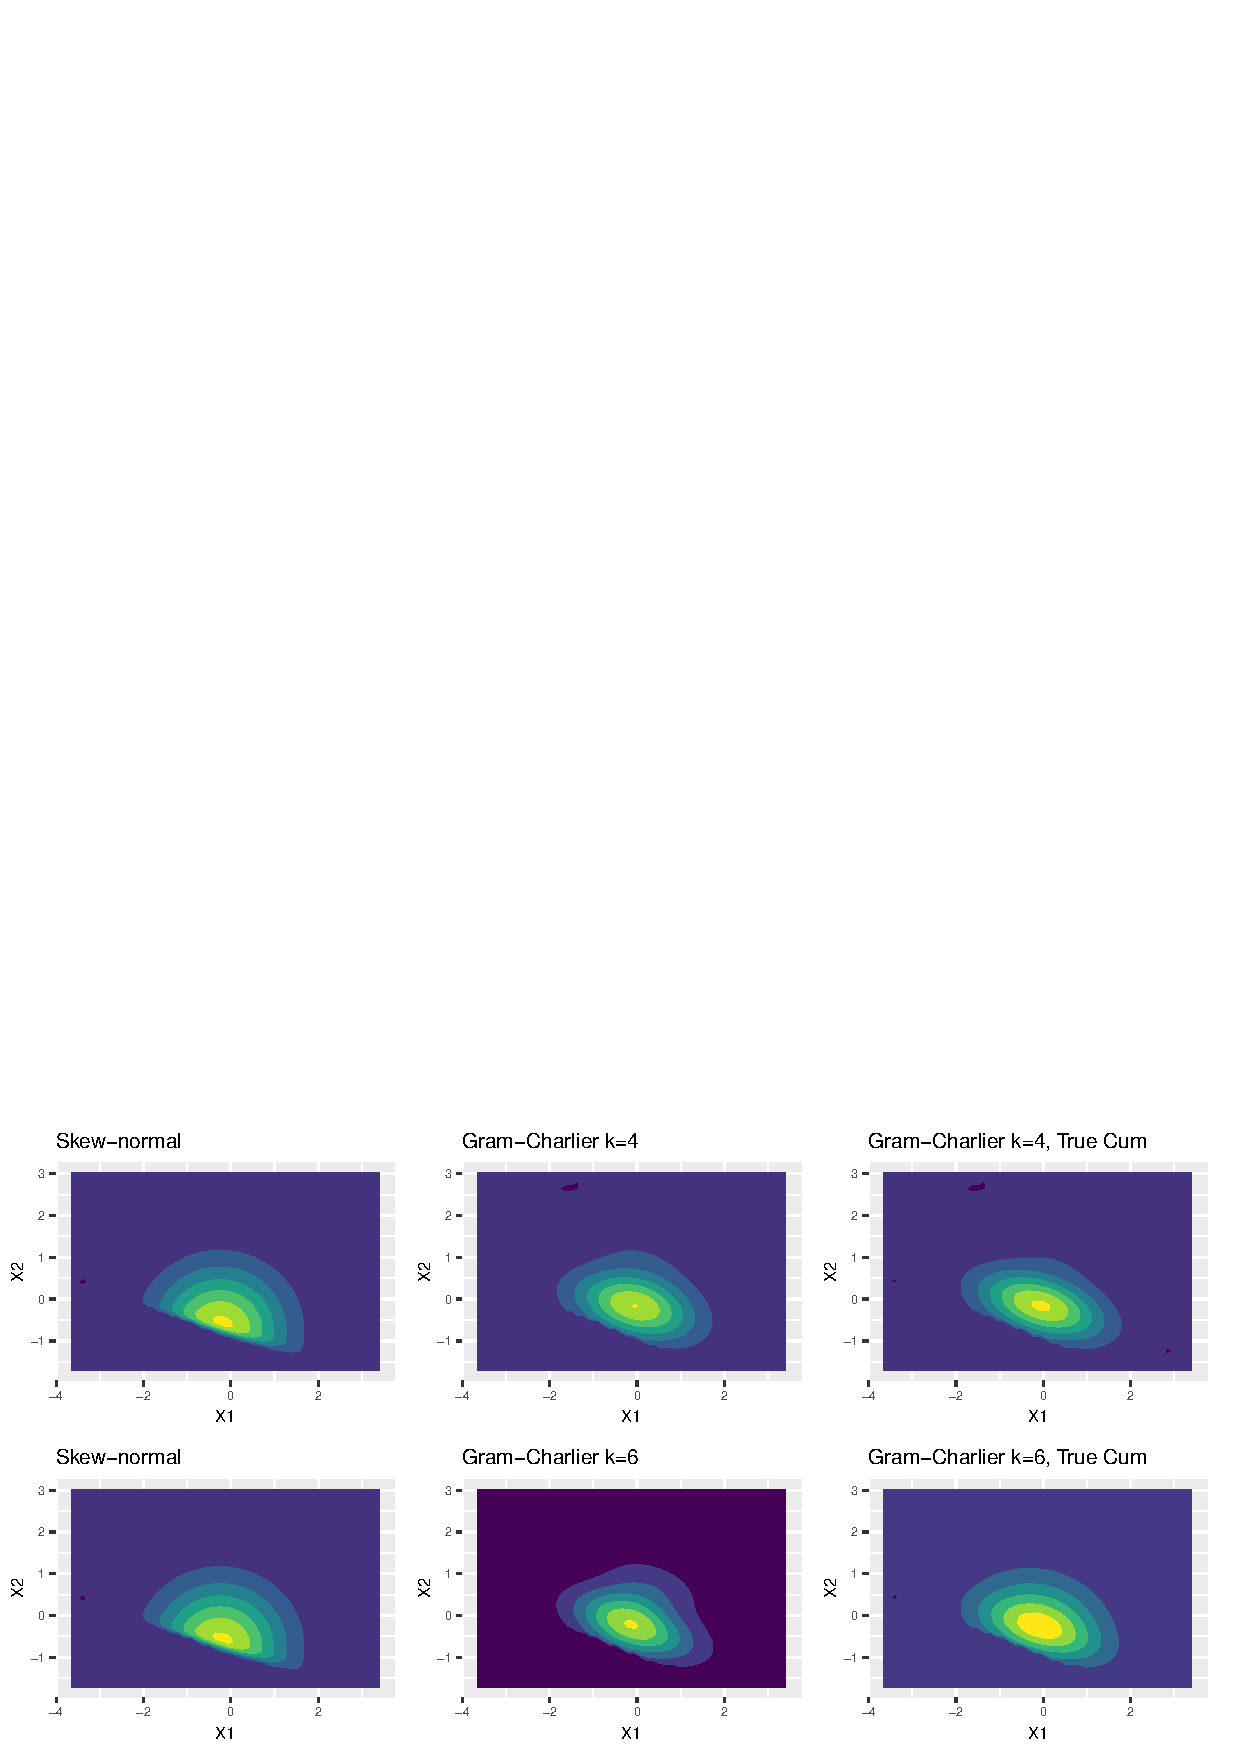
\includegraphics[width=1\linewidth,height=0.5\textheight]{figures/GCALL} \caption{Contour plots of the skew-normal true density (left), the Gram-Charlier approximation with estimated cumulants (center) and the Gram-Charlier approximation with true cumulants (right). Case with $k=4$ (first row) and $k=6$ (second row).}\label{fig:Gram-Charlier}
\end{figure}

\hypertarget{computational-details}{%
\section{Computational details}\label{computational-details}}

One of the basic functions of \CRANpkg{MultiStatM} is \texttt{PartitionTypeAll} (Section 2.1) whose algorithm to generate all partitions of the set \(1:N\) is based on the recursive generation of inclusive and exclusive partition matrices as described in \citet{terdik2021multivariate}, section 1.4. For example, the number of partitions of a given type \texttt{S\_r\_j} and \texttt{eL\_r} - see Section 2.1 produced by \texttt{PartitionTypeAll} are exploited in conversion formulae from moments to cumulants and viceversa. Recall that the conversion formula from moments to cumulants (\citet{terdik2021multivariate}, Section 3.4)) is given by
\begin{equation}
\begin{split}
\boldsymbol{\mu}_{n}^\otimes &= \sum_{{\cal{K}} \in {\cal{P}}_n} \mathbf{K}^{-1}_{p({\cal{K}})} \prod^\otimes_{b_j \in {\cal{K}}} \kappa^\otimes_{|b_j|}\\
  &= \mathbf{S}_{d \mathbf{1}_n}\left( \sum_{r=1}^n \sum_{\sum l_j =r, \sum j l_j = n} \frac{n!}{\prod_{j=1}^n l_j! (j!)^{l_j}} \prod_{j=1:n-r+1}^\otimes \kappa^{\otimes l_j}_j\right)
\end{split}
\label{eq:mtc}
\end{equation}
where the summation is over all partitions \({\cal{K}} = \{b_1, b_2,\dots, b_k\}\) of \(1 : n\); \(|b_j|\) denotes the cardinality of block \(b_j\). The simpler second formula, exploiting the symmetrizer matrix, derives from symmetry of \(\boldsymbol{\mu}_{n}^\otimes\).

As far as the formula from cumulants to moments (\citet{terdik2021multivariate}, Section 3.4) is concerned,
\begin{equation}
\boldsymbol{\kappa}_{n}^\otimes  
  = \mathbf{S}_{d \mathbf{1}_n}\left( \sum_{r=1}^n (-1)^{r-1} (r-1)!\sum_{\sum l_j =r, \sum j l_j = n}  \prod_{j=1:n-r+1}^\otimes \frac{1}{{l_j}!}\left( \frac{1}{j!}\boldsymbol{\mu}^{\otimes}_j\right)^{l_j}\right).
\label{eq:ctm}
\end{equation}
One can also use T-Bell polynomials \(\mathbf{B}_{n}\), and incomplete T-Bell polynomial \(\mathbf{B}_{n,r}\) (see, e.g.~Section 1.4.2 and Section 4.7 in \citet{terdik2021multivariate})
to show the structure of partitions in \eqref{eq:mtc} as
\begin{equation}
\boldsymbol{\mu }_{n}^{\otimes }=\mathbf{S}_{d \mathbf{1}_n} \mathbf{B}_{n}\left( \boldsymbol{%
\kappa }_{1}^{\otimes },\boldsymbol{\kappa }_{2}^{\otimes },\boldsymbol{\ldots },\boldsymbol{\kappa }_{n}^{\otimes }\right)
\end{equation}
and in \eqref{eq:ctm},
\begin{equation}
\boldsymbol{\kappa }_{n}^{\otimes }= \mathbf{S}_{d \mathbf{1}_n} \sum_{r=1}^{n}\left(
-1\right) ^{r-1}(r-1)!\mathbf{B}_{n,r}\left( \boldsymbol{\mu }_{1}^{\otimes },\boldsymbol{\ldots },\boldsymbol{\mu }_{n}^{\otimes }\right). 
\end{equation}
Consider now the symmetrizer matrix (Section 2.2), note that, by definition, its computation requires \(q!\) operations; in the package, the computational complexity is overcome by exploiting the \citet{Chacon2014} efficient recursive algorithms for functionals based on higher order derivatives and the prime factorization theorem. Note however that even though the computational requirements are greatly reduced, the symmetrizer is a square matrix of dimension \(d^n\) where \(d\) is the vector dimension and \(n\) the power of the Kronecker products. Since \texttt{SymMatr} produces essentially sparse matrices, the option \texttt{useSparse=T,F} can be selected (\texttt{F} is the default). Overall however, if the use of matrices is not strictly necessary, the function \texttt{SymIndx} will directly produce a symmetrized version of the T-product of vectors. Table \ref{tab:Symmetr} reports the computational times as well as memory allocation of the objects created. Computation times are approximate and obtained on a desktop computer with an Intel-Core-i7-7700 CPU at 3.60GHz and 16GB RAM. From the table it can be noted that using sparse matrices can be much faster and more efficient in terms of memory allocation. The use of \texttt{SymIndx} should be the standard way however, as it much less demanding in terms of memory allocation. Recall Example 3 for an instance where the use of \texttt{SymMatr} is preferable. The numerical results are in line with those of \citet{Chacon2014}.

In general the functions of the group \texttt{Indx} should be used wherever possible, as they are typically much faster than the corresponding \texttt{Matr} group since the former avoids constructing possibly large matrices. All code in \CRANpkg{MultiStatM} wherever possible, exploits the \texttt{Indx} group of functions.

\begin{longtable}[]{@{}llrr@{}}
\caption{\label{tab:Symmetr} Approximate memory allocation (in Kb or Mb) and computational times in secs (s) or mins (m) of \texttt{SymMatr} and \texttt{SymIndx} under different settings. For \(d=3\), \(n\) indicates the power of the Kronecker products.}\tabularnewline
\toprule\noalign{}
\textbf{Function} & \textbf{n} & \textbf{Time} & \textbf{Object size} \\
\midrule\noalign{}
\endfirsthead
\toprule\noalign{}
\textbf{Function} & \textbf{n} & \textbf{Time} & \textbf{Object size} \\
\midrule\noalign{}
\endhead
\bottomrule\noalign{}
\endlastfoot
SymMatr() & 4 & 0.003s & 55Kb \\
useSparse=F & 6 & 0.720s & 4Mb \\
& 8 & 9.2m & 344Mb \\
& & & \\
SymMatr() & 4 & 0.03s & 9Kb \\
useSparse=T & 6 & 0.12s & 0.4Mb \\
& 8 & 0.46s & 25Mb \\
& & & \\
Symindx() & 4 & 0.06 & 0.6Kb \\
& 6 & 0.02 & 0.6Kb \\
& 8 & 0.06 & 52Kb \\
\end{longtable}

A further discussion is needed for \texttt{CommutatorMatr} with \texttt{Type="Kperm"} (Section 2.2) which produces permutations of any \(\operatorname{T}\)-products of vectors of any dimensions: beyond the considerations concerning using \texttt{useSparse=T} or not, when using \texttt{CommutatorMatr} with \texttt{Type="Kperm"}, the dimensions of the vectors in the argument may have a large impact on computing time.

Recall that \texttt{CommutatorMatr} with \texttt{Type="Kperm"} produces a permutation \texttt{perm} of vectors of dimensions specified in \texttt{dims}. As an example consider the case of the product of \(n=8\) vectors all with the same dimension \(d\); using \texttt{dims\ \textless{}-\ d} instead of \texttt{dims\ \textless{}-\ c(d,d,d,d,d,d,d,d)} will require much less computing time. In the evaluation below

\begin{verbatim}
CommutatorMatr(Type = "Kperm", perm = c(2, 4, 6, 1, 3, 8, 5, 7), dims = 3)
\end{verbatim}

requires approximately 2.11 seconds while

\begin{verbatim}
CommutatorMatr(Type = "Kperm", perm = c(2, 4, 6, 1, 3, 8, 5, 7), 
               dims = c(3, 3, 3, 3, 3, 3, 3, 3))
\end{verbatim}

requires approximately 1326.47 seconds.

\bigskip

\textbf{Acknowledgement}. The work of Gy. H. Terdik has been supported by the project TKP2021-NKTA of the University of Debrecen, Hungary.
Project no. TKP2021-NKTA-34 has been implemented with the support provided by the Ministry of Culture and Innovation of Hungary from the National Research, Development and Innovation Fund, financed under the TKP2021-NKTA funding scheme.

\bibliography{RJreferences.bib}

\address{%
György Terdik\\
University of Debrecen\\%
Department of Informatics\\ Debrecen, Hungary\\
%
%
\textit{ORCiD: \href{https://orcid.org/0000-0002-9663-6892}{0000-0002-9663-6892}}\\%
\href{mailto:terdik.gyorgy@inf.unideb.hu}{\nolinkurl{terdik.gyorgy@inf.unideb.hu}}%
}

\address{%
Emanuele Taufer\\
University of Trento\\%
Department of Economics and Management\\ Trento, Italy\\
%
%
\textit{ORCiD: \href{https://orcid.org/0000-0001-5140-9912}{0000-0001-5140-9912}}\\%
\href{mailto:emanuele.taufer@unitn.it}{\nolinkurl{emanuele.taufer@unitn.it}}%
}
